\documentclass[a4paper, 12pt]{article}
\usepackage[hidelinks]{hyperref}
\usepackage[parfill]{parskip}
\usepackage{xfrac}
\usepackage[a4paper]{geometry}
\hypersetup
	{ pdfauthor={Magnar Myrtveit}
	, pdftitle={TempoWiki}
	, pdfsubject={An App for handling custom metadata for tracks in Spotify}
	}
\title{TempoWiki}
\author{Magnar Myrtveit}

\begin{document}
\begin{description}
\item[App Name] \hfill \\
TempoWiki
\item[Name] \hfill \\
Magnar Myrtveit
\item[E-mail] \hfill \\
\href{mailto:magnar@myrtveit.com}{magnar@myrtveit.com}
\item[Company and Website] \hfill \\
Not applicable
\item[Short description] \hfill \\
TempoWiki is an App for discovering music suitable for dancing. The user can search for music matching specific attributes:
\begin{itemize}
\item Dance genres the music should be suitable for
\item A tempo interval for how fast the music should be
\item The preferred music genres 
\end{itemize}
TempoWiki creates a playlist containing tracks matching the specified attributes for the user. Users can contribute to TempoWiki by registering metadata for tracks they like dancing to, in order to make the tracks available through TempoWiki.
\item[Long description]
\end{description}
\section{Introduction}
Spotify is a great resource for listening to your favourite music, in addition to discovering new music. However, finding music fitting specific criteria can be very difficult. If I am looking for Swing Jazz music around 56 bars suitable for dancing Balboa, my best guess would be to search for some user's balboa playlist and play through it until I hopefully find a track matching my criteria. I could create a playlist containing the tracks I've discovered, but the combination of different criteria makes it hard to create good and useful playlists; sometimes I want faster or slower music, sometimes I prefer Dixieland music, and sometimes I'd rather dance Lindy Hop than Balboa! After a while I'm probably even bored of dancing to the same tracks over and over again, and want some new danceable music. Then I have to start listening to people's playlists again, looking for new suitable music.

These are some of the difficulties I am aiming to resolve through TempoWiki. Instead of creating playlists containing danceable music, a user can register metadata for the tracks he or she likes dancing to. When a user is looking for music suitable for a specific dance genre, in a specific tempo interval, and of a specific music genre, TempoWiki can automatically create such a playlist based on metadata registered by TempoWiki users.

Being able to search for tracks of a specific tempo is very useful when looking for danceable music. Because of this most dance instructors use their own mp3 collection instead of Spotify when teaching. Their mp3 collection gives them the ability to enter tempo information for each track in the filename or track title, while Spotify lacks this feature. In addition to showing tempo information for tracks, TempoWiki allows for sorting the playlists by tempo. I believe this feature will make TempoWiki a great resource for dance instructors. Because I consider the ability to retrieve tempo information for a track and that the users themselves are building the metadata database as core features of this App, I chose to name it TempoWiki.

\section{User interface}
\label{sec:user-interface}
To make the application simple to use, TempoWiki uses strong visual components for as much of the user interaction as possible. It is much easier to click the button for the dance genre you are looking for than to type in the name of the dance, even with good auto complete functionality. Reuse of the visual components across all the different views of the application makes it easy to get familiar with the user interface and avoid confusion by controls being rearranged when going from one view to another. Most of the controls for user interaction regarding musical qualities are identical between the \hyperref[sec:playlist]{Playlist creator}, \hyperref[sec:player]{Now playing}, and \hyperref[sec:editor]{Metadata editor}. To prevent the user interface from becoming cluttered, the user can create custom profiles using the \hyperref[sec:profiler]{Profile creator}. In a profile, the user can tailor which properties and attributes are needed, and hence which controls should be visible in the user interface. For example, a Swing profile can be created where only the Swing dance genres the user likes to dance and the musical genres applicable to Swing dancing are displayed. If the user likes dancing Salsa as well, another profile only containing the controls needed when looking for Salsa music can be created.

\begin{figure}[placement h]
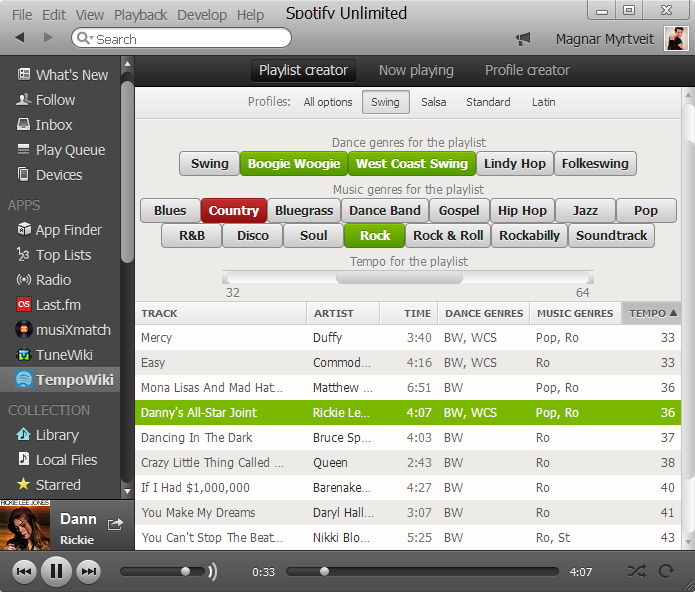
\includegraphics{img/user-interface.png}
\end{figure}

\section{Functionality}
\subsection{Now playing}
\label{sec:player}
In this view the \hyperref[sec:fetching]{metadata registered} (if any) for the currently playing track is displayed. The user can confirm that he or she agrees to the metadata registered to give this information a vote, or choose to edit the information if he or she does not fully agree to the metadata already registered.

If no tempo information has been registered for the currently playing track yet, tempo information is attempted retrieved from The Echo Nest. Tempo information is not available for all tracks through The Echo Nest, and sometimes the tempo is doubled or halved (or just totally off) and must be corrected manually in the \hyperref[sec:editor]{Metadata editor}. Most of the time the tempo information from The Echo Nest is very accurate, which makes registering tempo information for a track much easier.

\begin{figure}[placement h]
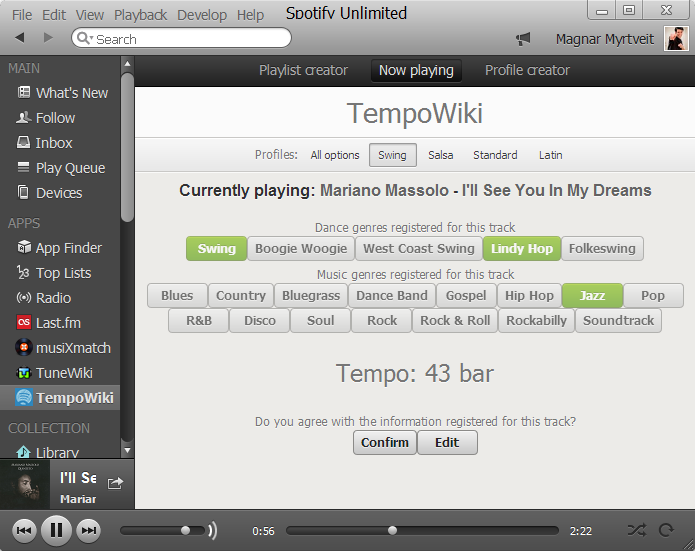
\includegraphics{img/now-playing.png}
\end{figure}

\subsection{Metadata editor}
\label{sec:editor}
The Metadata editor is where the actual track information is registered. When metadata has been registered for a track, the track may appear in playlists created using the \hyperref[sec:playlist]{Playlist creator}. When the Metadata editor is opened, the \hyperref[sec:fetching]{metadata already registered} (if any) for the edited track is displayed. This information can then be altered and saved by the user.

\begin{figure}[placement h]
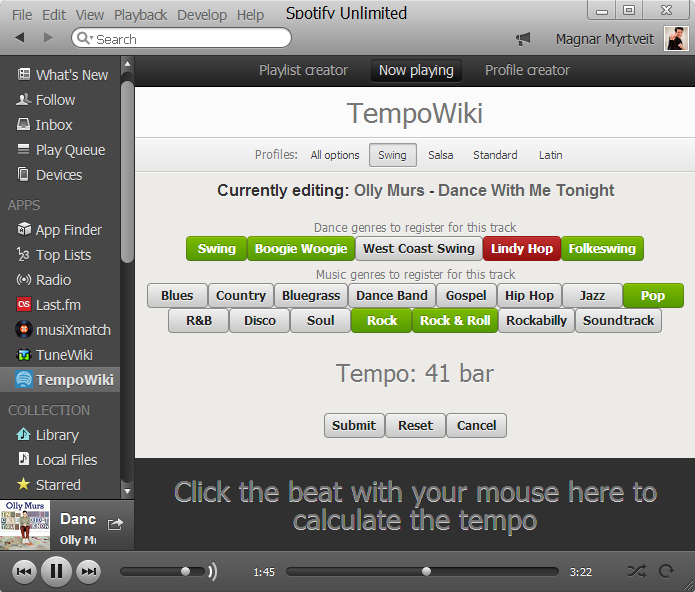
\includegraphics{img/metadata-editor.png}
\end{figure}

To register the tempo information for a track, the user can click the beat using the mouse while the track is playing. TempoWiki registers the interval between each click, and calculates the track's tempo.

The button controls in the Metadata editor can be either two-state or three-state buttons. For a button for the attribute X, the different states have the following meanings:
\begin{description}
	\item[State 1] The user does not consider X as applicable for the track, but it is ok for the track to be displayed in playlists when searching for tracks with the attribute X if most other users regard X as applicable for the track.
	\item[State 2] The user thinks X applies to the track.
	\item[State 3] The user does not consider X as applicable for the track, and the track should not be displayed in playlists when searching for tracks with the attribute X even if most other users regard X as applicable for the track.
\end{description}
Most of the time only State 1 and State 2 will be needed. State 3 should not be used except for tracks that show up in playlists where they, in the user's opinion, do not belong. For example, it is generally not necessary to set the button for Rockabilly to State 3 instead of State 1 when registering metadata for a Soul track, as most other users are not likely to regard the track as Rockabilly, so it will never appear in a Rockabilly playlist anyway.
\subsection{Playlist creator}
\label{sec:playlist}
For the normal user, this will be the most used view of the application, where playlists are created based on the user's criteria. Just specify what kind of music you are looking for using the controls, and a playlist will be generated.

The button controls in the Playlist creator can be either two-state or three-state buttons. For a button for the attribute X belonging to the property Y, the different states have the following meanings:
\begin{description}
	\item[State 1] X is not considered when creating the playlist.
	\item[State 2] For every track in the playlist, X or any other attribute belonging to Y whose button is currently in State 2 should apply.
	\item[State 3] X should not apply to any of the tracks in the playlist.
\end{description}
For example, if the property Dance genres is set to use three-state buttons, if I click the buttons ``Boogie Woogie'' and ``West Coast Swing'', a playlist where all the tracks are suitable for dancing Boogie Woogie or West Coast Swing is created. Some of these tracks might also be suitable for dancing Lindy Hop. If I click the button ``Lindy Hop'' twice, the tracks suitable for dancing Lindy Hop will not be displayed, even though they are suitable for dancing Boogie Woogie or West Coast Swing.

The \hyperref[sec:fetching]{metadata registered} for the tracks is displayed in the playlists. Genres are displayed in short versions, and the long versions are displayed on mouseover. To increase the credibility of the metadata registered for the tracks, it should be easy to confirm or edit the registered information. I am planning on displaying two buttons on each row of the playlist. When clicking the Agree button, the user's vote is registered to confirm the metadata\footnote{Only the metadata that is displayed in the active \hyperref[sec:profiler]{profile} is registered} registered for the track. If the Disagree button is clicked, the \hyperref[sec:editor]{Metadata editor} is displayed, allowing the user to register which metadata he or she thinks is most applicable for the track.

The playlist can be sorted by clicking on the header for the property you would like to sort by. Not all properties are sortable.

\begin{figure}[placement h]
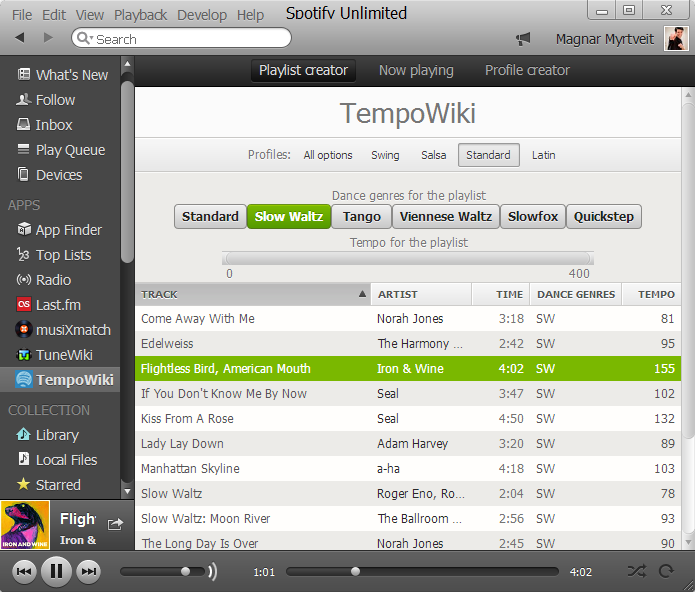
\includegraphics{img/playlist-creator.png}
\end{figure}

\subsection{Profile creator}
\label{sec:profiler}
Using the Profile creator, the user can specify exactly which controls are needed when searching for different kinds of music. If a user is only interested in music for dancing Swing and Salsa, a profile can be created that hides all controls not related to Swing or Salsa music. If the user has no need to search for both Swing and Salsa music at the same time, the user interface can be made even cleaner by creating separate profiles for when he or she is looking for Swing and Salsa music. Which units should be used for measuring tempo can also be specified in the profiles. For example, bars are mainly used when dealing with Swing music, while Standard music is always measured in bpm. Which units should be available can be specified for each profile, in addition to the profile's applicable tempo range.

I think profiles is one of the most important features for TempoWiki to become a success. Without profiles I believe most users would find the \hyperref[sec:user-interface]{user interface} too cluttered and complicated. With profiles the user can clean up the user interface and make it more appealing. Each user can increase the usability and relevancy of TempoWiki by tailoring the user interface towards his or her needs. But it might become a challenge to make users understand what the profiles do, and to help first-time users set up their first profiles. I am considering creating an interactive tutorial that will be run whenever a new user starts using TempoWiki, helping users to create their first profile and their first playlist.
\section{How a track's metadata is calculated}
\label{sec:fetching}
When fetching metadata for a track, all metadata (if any) registered by the current user for the track is fetched. For properties where the user has not registered any metadata, the value the majority of the users agree upon is fetched. For instance, if a user has registered tempo information and dance genres, but not music genres (music genres was not being displayed in the profile used when registering metadata for the track), the tempo and dance genre information registered by the user is fetched, while the fetched music genre information will be based on metadata registered by other users. This also applies to attributes within a property. If the user has registered dance genre metadata for a track but the genre Charleston was not being displayed in the profile used during registration, the fetched dance genre information will be what the user registered for the track, but whether Charleston applies to the track or not will be based on metadata registered by other users. Because of this it is ok for users to disagree upon what metadata is applicable to a track, as other users' metadata registrations will never overrule the current user's metadata registrations.
\section{Current status}
\label{sec:status}
I have created a working beta version of TempoWiki. I am planning on using it when teaching dance lessons this semester, and I have also set up TempoWiki for a handful of other dancers for them to try out and give me some feedback. The beta version is not ready for mass distribution yet, as most users probably will not understand how it is used and what it can be used for without some introduction. But apart from missing an interactive guide to help first-time users understand the use of the application, TempoWiki is not very far from being ready for submission for approval. That's unless you notice loads of things that must be changed in order for TempoWiki to conform with the Spotify guidelines.

I hope you like the concept, and I'm looking forward to hearing from you.

Best regards,\\
Magnar Myrtveit
\end{document}